% report.tex - Переработанный отчёт по курсовой работе
\documentclass[a4paper, final]{extarticle}
\usepackage[russian]{babel}
\usepackage[utf8]{inputenc}
\usepackage[T2A]{fontenc}
\usepackage[14pt]{extsizes}
\usepackage[left=20mm, top=20mm, right=20mm, bottom=20mm, footskip=10mm]{geometry}
\usepackage{ragged2e}
\usepackage{indentfirst}
\usepackage{hyperref}
\usepackage{graphicx}
\usepackage{tikz}
\usetikzlibrary{positioning}
\usepackage{pdflscape}
\usepackage{pdfpages}
\usepackage{array}
\usepackage{booktabs}
\usepackage{listings}
\usepackage{xcolor}
\usepackage{amsmath}
\usepackage{amssymb}
\usepackage{caption}
\usepackage{subcaption}
\usepackage{float}
\usepackage{pifont}
\usepackage{cmap}
\usetikzlibrary{positioning,arrows.meta}

\definecolor{codegreen}{rgb}{0,0.6,0}
\definecolor{codegray}{rgb}{0.5,0.5,0.5}
\definecolor{codepurple}{rgb}{0.58,0,0.82}
\definecolor{backcolour}{rgb}{0.95,0.95,0.92}

\lstdefinestyle{mystyle}{
	commentstyle=\color{codegreen},
	keywordstyle=\color{magenta},
	numberstyle=\tiny\color{codegray},
	stringstyle=\color{codepurple},
	basicstyle=\ttfamily\footnotesize,
	breakatwhitespace=false,         
	breaklines=true,                 
	captionpos=b,                    
	keepspaces=true,                 
	numbers=left,                    
	numbersep=5pt,                  
	showspaces=false,                
	showstringspaces=false,
	showtabs=false,                  
	tabsize=2,
	inputencoding=utf8,
	extendedchars=true,
	literate={а}{{\selectfont\char224}}1
	{б}{{\selectfont\char225}}1
	{в}{{\selectfont\char226}}1
	{г}{{\selectfont\char227}}1
	{д}{{\selectfont\char228}}1
	{е}{{\selectfont\char229}}1
	{ё}{{\"e}}1
	{ж}{{\selectfont\char230}}1
	{з}{{\selectfont\char231}}1
	{и}{{\selectfont\char232}}1
	{й}{{\selectfont\char233}}1
	{к}{{\selectfont\char234}}1
	{л}{{\selectfont\char235}}1
	{м}{{\selectfont\char236}}1
	{н}{{\selectfont\char237}}1
	{о}{{\selectfont\char238}}1
	{п}{{\selectfont\char239}}1
	{р}{{\selectfont\char240}}1
	{с}{{\selectfont\char241}}1
	{т}{{\selectfont\char242}}1
	{у}{{\selectfont\char243}}1
	{ф}{{\selectfont\char244}}1
	{х}{{\selectfont\char245}}1
	{ц}{{\selectfont\char246}}1
	{ч}{{\selectfont\char247}}1
	{ш}{{\selectfont\char248}}1
	{щ}{{\selectfont\char249}}1
	{ъ}{{\selectfont\char250}}1
	{ы}{{\selectfont\char251}}1
	{ь}{{\selectfont\char252}}1
	{э}{{\selectfont\char253}}1
	{ю}{{\selectfont\char254}}1
	{я}{{\selectfont\char255}}1
	{А}{{\selectfont\char192}}1
	{Б}{{\selectfont\char193}}1
	{В}{{\selectfont\char194}}1
	{Г}{{\selectfont\char195}}1
	{Д}{{\selectfont\char196}}1
	{Е}{{\selectfont\char197}}1
	{Ё}{{\"E}}1
	{Ж}{{\selectfont\char198}}1
	{З}{{\selectfont\char199}}1
	{И}{{\selectfont\char200}}1
	{Й}{{\selectfont\char201}}1
	{К}{{\selectfont\char202}}1
	{Л}{{\selectfont\char203}}1
	{М}{{\selectfont\char204}}1
	{Н}{{\selectfont\char205}}1
	{О}{{\selectfont\char206}}1
	{П}{{\selectfont\char207}}1
	{Р}{{\selectfont\char208}}1
	{С}{{\selectfont\char209}}1
	{Т}{{\selectfont\char210}}1
	{У}{{\selectfont\char211}}1
	{Ф}{{\selectfont\char212}}1
	{Х}{{\selectfont\char213}}1
	{Ц}{{\selectfont\char214}}1
	{Ч}{{\selectfont\char215}}1
	{Ш}{{\selectfont\char216}}1
	{Щ}{{\selectfont\char217}}1
	{Ъ}{{\selectfont\char218}}1
	{Ы}{{\selectfont\char219}}1
	{Ь}{{\selectfont\char220}}1
	{Э}{{\selectfont\char221}}1
	{Ю}{{\selectfont\char222}}1
	{Я}{{\selectfont\char223}}1
	{/}{{\selectfont\char224}}1
	{—}{{\selectfont\char225}}1
	{«}{{\selectfont\char226}}1
	{»}{{\selectfont\char227}}1
	{№}{{\selectfont\char228}}1
	{–}{{\selectfont\char229}}1,
}

\lstset{style=mystyle}

\begin{document}
	
	{\thispagestyle{empty}
		\begin{center}
			\hfill \break
			\hfill \break
			Министерство образования и науки Российской Федерации\\[3pt]
			Санкт-Петербургский политехнический университет Петра Великого\\[10pt]
			Институт компьютерных наук и кибербезопасности\\[3pt]
			Высшая школа технологий искусственного интеллекта\\[3pt]
			Направление: 02.03.01 «Математика и компьютерные науки»\\
			[110pt]
			
			\large Отчёт о выполнении курсовой работы\\[5pt]			
			\large по дисциплине \flqq Теория графов\frqq \\[5pt]
			\large на тему:\\[5pt] 		
			\large \flqq Экспертная система определения типа аллергии\frqq \\[5pt]
		\end{center}
		
		\vspace{90 pt}
		
		\begin{tabular*}{460pt}{@{\extracolsep{\fill}} l r l}
			Выполнил студент\tabularnewline группы 5130201/40002 & \hspace{55pt} \line(1,0){100} \hspace{-35pt} & Алексеев Л. К.\\
			& \\
			Проверил \tabularnewline преподаватель & \hspace{55pt} \line(1,0){100} \hspace{-35pt} & \hfill Востров А. В. \\
			& \\
			& \\
			& \\
			& \multicolumn{2}{r}{\guillemotleft \line(1,0){30} \guillemotright \line(1,0){100} \, 2026г.}
			
		\end{tabular*} \\
		
		\vfill
		
		\centering Санкт-Петербург
		
		\centering 2026
		
		\newpage
	}
	
	\tableofcontents
	\newpage
	
	\section*{Введение}
	\addcontentsline{toc}{section}{Введение}
	
	Целью курсовой работы является разработка экспертной системы, основанной на продукционной модели представления знаний, для определения типа аллергии по симптомам пользователя. Система реализована в среде CLIPS и использует бинарное дерево решений для интерактивного опроса пользователя и вывода наиболее вероятного типа аллергии. В отчёте приведены математическое описание используемых моделей, особенности реализации и результаты тестирования.
	
	\newpage
	
	\section{Постановка задачи}
	
	Для достижения цели были сформулированы следующие задачи:
	\begin{enumerate}
		\item Выбрать предметную область и утвердить с преподавателем;
		\item Сформулировать критерии для экспертной системы;
		\item Разработать диаграмму для экспертной системы;
		\item Реализовать экспертную систему в среде CLIPS;
	\end{enumerate}
	
	\newpage
	
	\section{Предметная область}
	
	Аллергия — патологическая реакция иммунной системы на внешние или внутренние раздражители (аллергены). Тип аллергии определяется по совокупности симптомов: кожные проявления, респираторные симптомы, желудочно-кишечные реакции, связь с контактами и сезонностью.
	
	В системе Используются следующие критерии для выявления типа аллергии (всего 25 критериев):
	\begin{itemize}
		\item Реакция возникает в течение 1–12 часов после контакта с аллергеном?
		\item В анамнезе есть указания на перенесённую тяжёлую системную реакцию (анафилаксию)?
		\item Реакция возникает не менее чем через 12 часов после контакта с аллергеном?
		\item Реакцию вызвало жалящее насекомое?
		\item Реакция связана с дыхательной системой?
		\item Реакция связана с кожей (например, сыпь, зуд)?
		\item Реакция всегда возникает на холод/тепло/солнце?
		\item Реакция возникла во время или после внутривенного введения лекарства?
		\item Симптомы (чихание, зуд, ринорея) появляются сезонно во время цветения?
		\item Реакция проявляется на коже?
		\item Сыпь появилась в месте нанесения мази/пластыря или контакта с одеждой с металлическими деталями?
		\item Реакция проявилась в виде лихорадки, болей в суставах после укуса насекомого?
		\item Симптомы (волдыри, зуд, покраснение) появляются под воздействием провоцирующего фактора?
		\item Симптомы начались в течение 30 минут после употребления \\ арахиса/орехов/моллюсков?
		\item Симптомы сохраняются круглый год и усиливаются дома или на работе?
		\item При контакте с аллергеном возникают зуд, волдыри, покраснение?
		\item Реакция связана с желудочно-кишечным трактом (ЖКТ)?
		\item Сыпь генерализованная, появилась через несколько дней после приёма внутрь антибиотиков, например пенициллина?
		\item Основной симптом — приступы удушья, свистящее дыхание?
		\item Сыпь появилась через 12–48 часов после контакта с металлом/косметикой, похожа на экзему?
		\item Симптомы (боль в животе, тошнота, рвота, диарея) возникают у ребёнка до 2 лет при употреблении коровьего молока/яиц/сои?
		\item Реакция возникает при физической нагрузке?
		\item Беспокоят спонтанно возникающие зудящие волдыри («крапивница»), длятся менее 24 часов?
		\item Симптомы ЖКТ появляются через несколько часов после употребления пшеницы/морепродуктов?
		\item Симптомы появляются только после еды перед физической нагрузкой?
	\end{itemize}
	
	
	
	\newpage

	
	\section{Математическое описание}
	
	\subsection{Экспертные системы}
	
	Экспертная система — это программный комплекс, предназначенный для анализа проблемных ситуаций и выдачи рекомендаций, частично заменяя эксперта-человека. Выделяют два режима работы:
	\begin{enumerate}
		\item \textbf{Режим приобретения знаний} — наполнение системы знаниями при участии эксперта и инженера по знаниям.
		\item \textbf{Режим решения задачи (консультационный)} — автономная работа системы, когда конечный пользователь вводит данные и получает решение с обоснованием.
	\end{enumerate}
	
	\subsection{Структура экспертной системы}
	
	Экспертная система состоит из следующих компонентов:
	\begin{itemize}
		\item \textbf{База знаний} — содержит правила вывода и информацию о предметной области.
		\item \textbf{Рабочая память (база данных)} — хранит факты, введённые пользователем и выведенные системой.
		\item \textbf{Механизм логического вывода} — определяет, какие правила применить и в каком порядке. Используются стратегии прямой цепочки рассуждений (от данных к заключению) или обратной цепочки.
	\end{itemize}
	
	\subsection{Продукционная модель представления знаний}
	
	Продукционная модель — способ организации знаний в виде правил \textbf{ЕСЛИ <условие>, ТО <действие>, ИНАЧЕ <действие>}. Каждое правило независимо, что обеспечивает модульность и лёгкость расширения. Достоинства модели: простота, прозрачность вывода, естественность для экспертов. Недостатки: сложность управления при большом числе правил, возможные конфликты, трудности с нечёткими данными.
	
	В разработанной системе используется прямая цепочка рассуждений: правила срабатывают при появлении в рабочей памяти факта \texttt{(next-node ...)}, который указывает текущий узел дерева.
	
	\subsection{Бинарное дерево решений}
	
	Дерево решений — это ациклический граф, где каждый узел соответствует проверке условия (вопросу), каждое ребро — ответу («да»/«нет»), а листья — конечным решениям (диагнозам). В данной системе дерево содержит 6 ярусов, более 30 узлов и 23 листа. Корневой вопрос о временном профиле реакции обеспечивает быстрое разделение клинических сценариев и уменьшает среднюю глубину поиска.
	
	Структура диагностического дерева представлена на рис. 1. Корнем является вопрос о временном профиле реакции (1–12 часов), что позволяет сразу разделить немедленные и отсроченные реакции.
	
	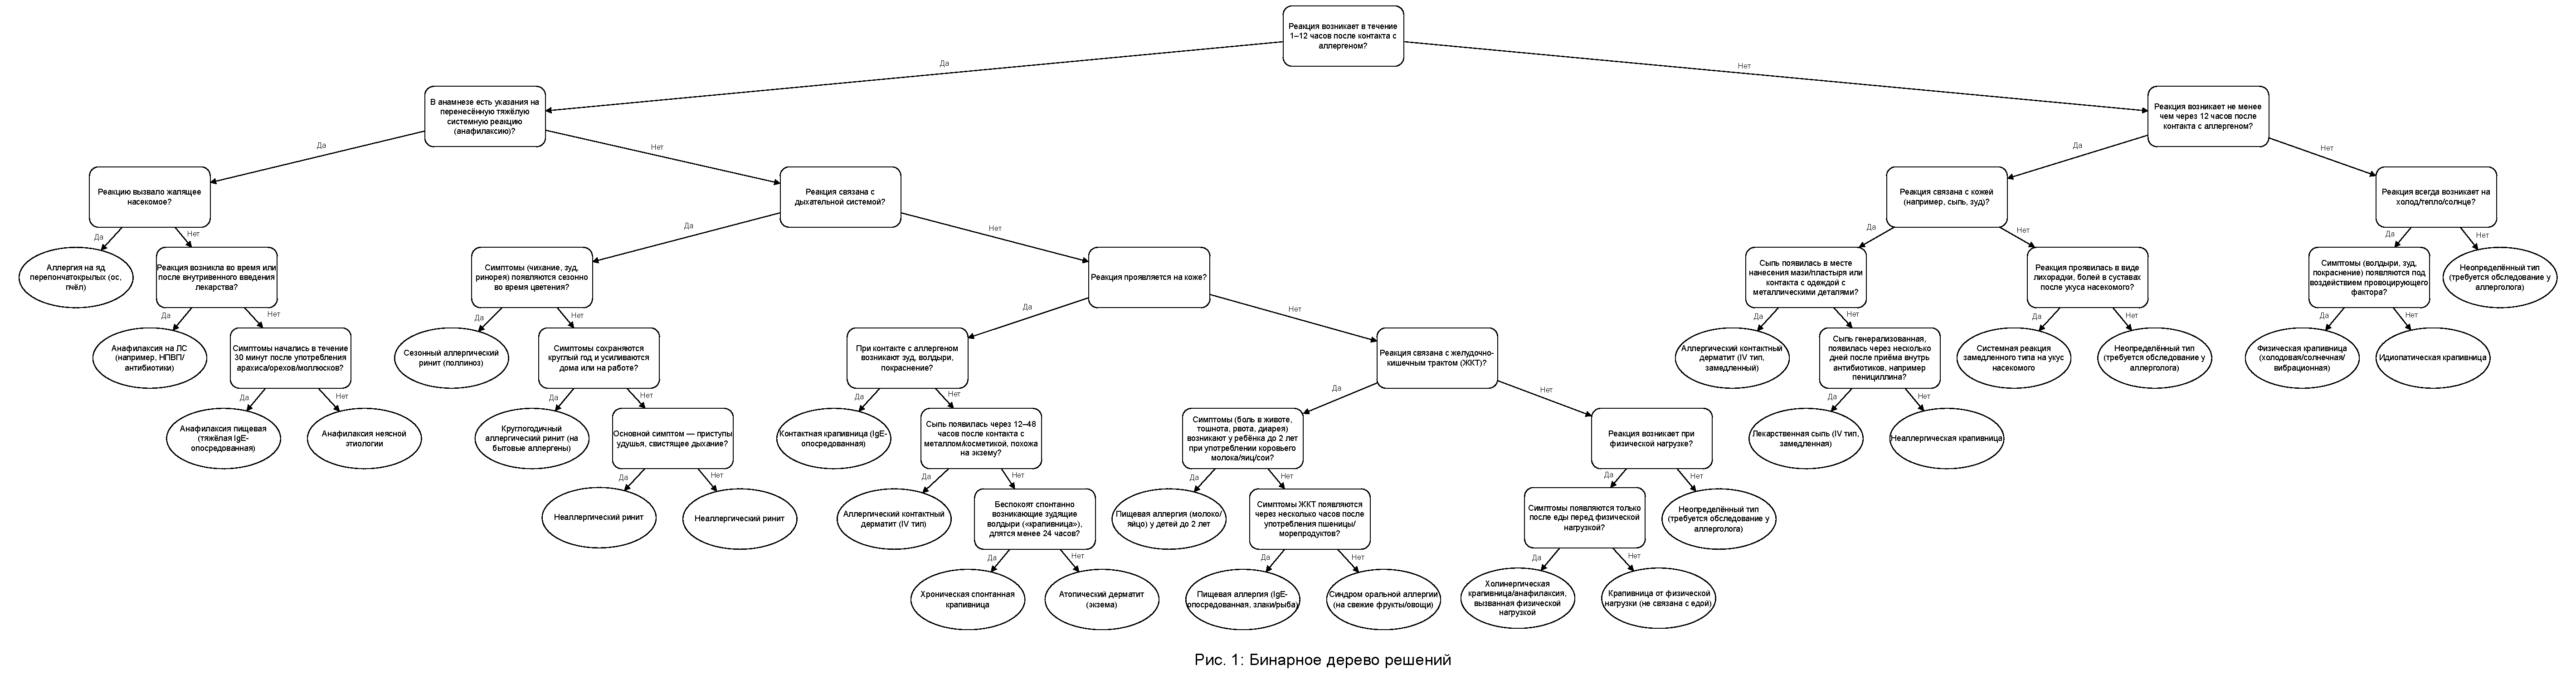
\includepdf[fitpaper]{Tree_allergy.drawio.pdf}
	
	\setcounter{figure}{1}
	
	\newpage
	
	\section{Особенности реализации}
	
	\subsection{Управление деревом решений с помощью \texttt{next-node}}
	
	Рабочая память содержит только один управляющий факт вида \texttt{(next-node <имя\_узла>)}, который указывает, какой узел диагностического дерева должен быть обработан в данный момент. Например, факт \texttt{(next-node q1)} означает, что следующим должен быть задан вопрос, соответствующий узлу \texttt{q1}.
	
	Переход по дереву выполняется путём добавления нового факта \texttt{(next-node ...)}. Старый факт при этом остаётся в рабочей памяти, но соответствующее правило уже не активируется повторно, так как его левая часть перестаёт быть истинной при сопоставлении с другими данными. Это позволяет системе последовательно обходить узлы дерева без явного удаления фактов.
	
	\subsection{Функция \texttt{ask-question}}
	
	Главный механизм взаимодействия с пользователем реализован в функции \texttt{ask-question}:
	
	\begin{lstlisting}
		(deffunction ask-question (?question ?yes-node ?no-node)
		(printout t ?question " (yes/no): ")
		(bind ?answer (read))
		(if (eq ?answer yes)
		then (assert (next-node ?yes-node))
		else (assert (next-node ?no-node))))
	\end{lstlisting}
	
	Она выводит текст вопроса, считывает ответ и, в зависимости от того, ввёл ли пользователь \texttt{yes} или любое другое слово (рассматриваемое как «нет»), добавляет в рабочую память факт \texttt{next-node} с именем следующего узла. Система не выполняет валидацию ввода, полагаясь на то, что пользователь сознательно вводит \texttt{yes} или \texttt{no}.
	
	\subsection{Отсутствие отдельных функций \texttt{member}}
	
	В отличие от некоторых других реализаций, данный код не использует функцию \texttt{member} для проверки ввода, поскольку ответы заведомо бинарны. Вся логика опроса сосредоточена в \texttt{ask-question}, которая непосредственно передаёт управление следующему узлу.
	
	\subsection{Правило инициализации \texttt{main-start}}
	
	Для запуска диагностики служит правило \texttt{main-start}:
	
	\begin{lstlisting}
		(defrule main-start
		(not (next-node ?))
		=>
		(assert (next-node q1)))
	\end{lstlisting}
	
	Оно срабатывает только при отсутствии в рабочей памяти любого факта \texttt{next-node} и устанавливает начальный узел \texttt{q1}.
	
	\subsection{Правила-вопросы (промежуточные узлы)}
	
	Каждый узел, соответствующий вопросу, реализован в виде отдельного правила. Левая часть правила содержит факт \texttt{(next-node <имя>)}. Правая часть вызывает \texttt{ask-question} с тремя аргументами: текстом вопроса, именем узла для ответа «да» и именем узла для ответа «нет». Пример для корневого вопроса:
	
	\begin{lstlisting}
		(defrule q1
		(next-node q1)
		=>
		(ask-question "Реакция возникает в течение 1–6 часов после контакта с аллергеном?" q2_yes q2_no))
	\end{lstlisting}
	
	После вызова \texttt{ask-question} в рабочую память добавляется факт \texttt{(next-node q2\_yes)} или \texttt{(next-node q2\_no)}, что активирует следующее правило.
	
	\subsection{Листовые правила (вывод диагноза)}
	
	Листья дерева представлены правилами, которые не вызывают \texttt{ask-question}, а сразу выводят диагноз и завершают работу системы. Никаких шаблонов типа \texttt{repair} для этого не используется. Пример листового правила:
	
	\begin{lstlisting}
		(defrule leaf_bee
		(next-node leaf_bee)
		=>
		(printout t "Диагноз: Аллергия на яд перепончатокрылых (ос, пчёл)" crlf)
		(printout t "--- Диагностика завершена ---" crlf)
		(halt))
	\end{lstlisting}
	
	Команда \texttt{(halt)} останавливает выполнение CLIPS, что полностью завершает сеанс диагностики.
	
	\subsection{Отсутствие глобального правила \texttt{print-result}}
	
	В системе нет отдельного правила \texttt{print-result} с низкой значимостью (salience). Каждое листовое правило самостоятельно выводит результат, что упрощает структуру программы и делает её более наглядной.
	
	\subsection{Общая схема работы}
	
	\begin{enumerate}
		\item При запуске правило \texttt{main-start} создаёт факт \texttt{(next-node q1)}.
		\item Активируется правило \texttt{q1}, которое через \texttt{ask-question} задаёт пользователю первый вопрос и создаёт факт \texttt{next-node} для следующего узла.
		\item Система последовательно переходит от узла к узлу, пока не достигнет листа.
		\item Листовое правило выводит диагноз и останавливает выполнение.
	\end{enumerate}
	
	Такой подход полностью соответствует продукционной модели прямой цепочки рассуждений и обеспечивает лёгкое расширение дерева добавлением новых правил без изменения существующего механизма вывода.
	
	\newpage
	
	\section{Результаты работы}
	
	Программа успешно реализует описанное бинарное дерево решений. Ниже приведены примеры сеансов работы для различных сценариев (скриншоты с рис. \ref{fig:food} по рис. \ref{fig:neopr}).
	
	\begin{figure}[H]
		\centering
		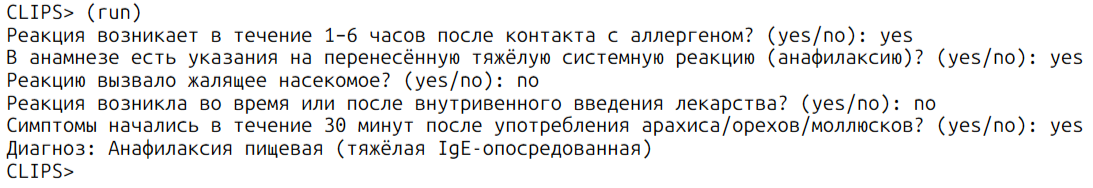
\includegraphics[width=1.0\textwidth]{pic/1.png}
		\caption{Получение диагноза: пищевая анафилаксия}
		\label{fig:food}
	\end{figure}
	
	\begin{figure}[H]
		\centering
		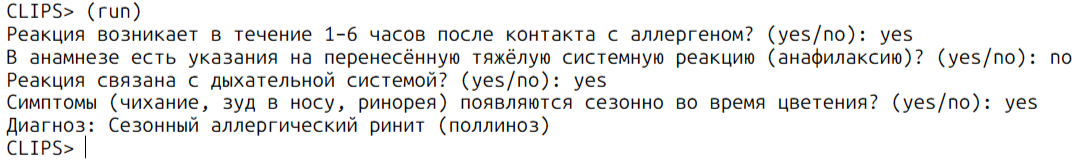
\includegraphics[width=1.0\textwidth]{pic/2.png}
		\caption{Получение диагноза: сезонный аллергический ринит (поллиноз)}
		\label{fig:nose}
	\end{figure}
	
	\begin{figure}[H]
		\centering
		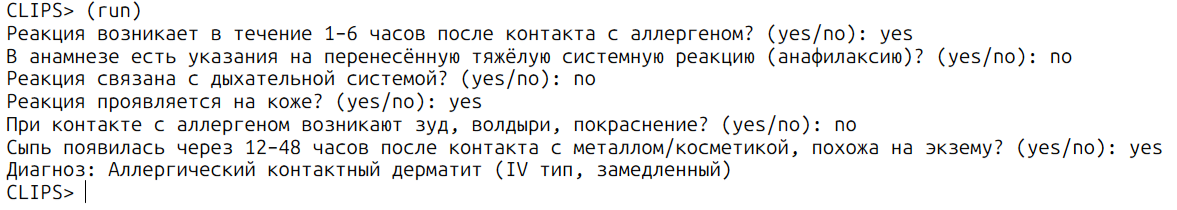
\includegraphics[width=1.0\textwidth]{pic/3.png}
		\caption{Получение диагноза: контактный дерматит}
		\label{fig:skin}
	\end{figure}
	
	\begin{figure}[H]
		\centering
		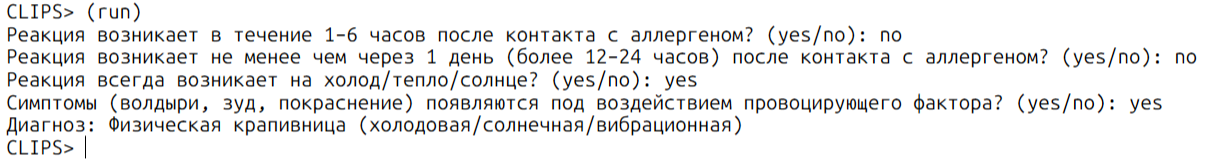
\includegraphics[width=1.0\textwidth]{pic/4.png}
		\caption{Получение диагноза: физическая крапивница}
		\label{fig:krapiva}
	\end{figure}
	
	Система также корректно обрабатывает неопределённые ситуации, выводя соответствующий лист «Неопределённый тип».
	
	\begin{figure}[H]
		\centering
		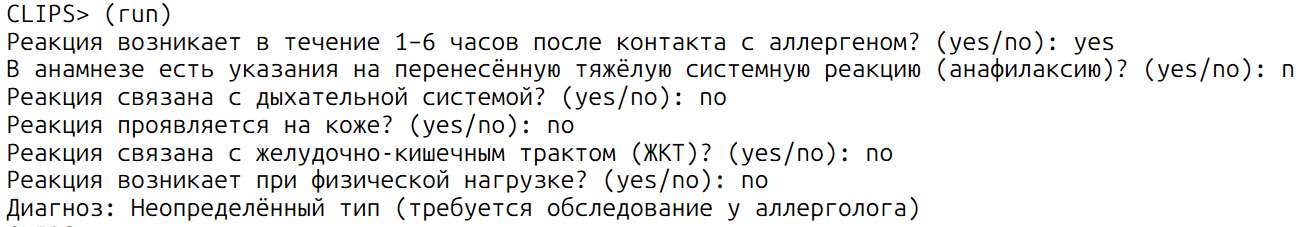
\includegraphics[width=1.0\textwidth]{pic/5.png}
		\caption{Вывод программы при неопределённом диагнозе}
		\label{fig:neopr}
	\end{figure}
	
	\newpage
	
	\section*{Заключение}
	\addcontentsline{toc}{section}{Заключение}
	
	Разработанная экспертная система полностью соответствует требованиям технического задания: она использует продукционную модель представления знаний, реализована в среде CLIPS, применяет бинарное дерево решений (6 ярусов, более 30 узлов) и выдаёт диагностические заключения на основе ответов пользователя.
	
	\paragraph{Программа предоставляет следующие возможности:}
	\begin{itemize}
		\item Интерактивный опрос пользователя с бинарными ответами (yes/no);
		\item Автоматическое перемещение по диагностическому дереву в зависимости от выбранных ответов;
		\item Вывод точного диагноза (один из 23 типов аллергических реакций) или рекомендацию обратиться к аллергологу при неопределённой картине;
	\end{itemize}
	
	\paragraph{Достоинства реализации:}
	\begin{itemize}
		\item Простота и наглядность кода — каждое правило соответствует одному узлу дерева, что упрощает отладку и верификацию;
		\item Сложность консультации для бинарного дерева составляет $O(\log n)$, что обеспечивает быстрое диагностирование при больших количествах диагнозов;
		\item Лёгкость расширения — для добавления нового вопроса или диагноза достаточно ввести новое правило и, при необходимости, связать его с существующими узлами;
		\item Прозрачность логического вывода — последовательность сработавших правил полностью соответствует пути по дереву решений.
	\end{itemize}
	
	\paragraph{Недостатки реализации:}
	\begin{itemize}
		\item Отсутствие валидации пользовательского ввода — система ожидает строго \texttt{yes} или \texttt{no}; любое другое слово интерпретируется как \texttt{no}, что может приводить к неверной ветке при опечатке;
		\item Невозможность объяснения вывода — после получения диагноза система не показывает, какие именно ответы привели к данному заключению;
		\item Отсутствие поддержки многовариантных ответов — все вопросы сформулированы как бинарные, хотя в некоторых клинических ситуациях полезны были бы варианты «не знаю» или «частично»;
	\end{itemize}
	
	\newpage
	
	\addcontentsline{toc}{section}{Список литературы}
	\begin{thebibliography}{9}
		\bibitem{novikov} Новиков Ф.А. Дискретная математика для программистов. 3-е изд. – Санкт-Петербург: Питер Пресс, 2009. – 384 с.
		\bibitem{clips} CLIPS — \textit{CLIPS User's Guide and Reference Manual}. Официальная документация CLIPS. Доступно: \url{https://www.clipsrules.net/}.
		\bibitem{who} Всемирная организация здравоохранения. \textit{МКБ-11 для ведения статистики смертности и заболеваемости}. Доступно: \url{https://icd.who.int/browse/2025-01/mms/ru}.
		\bibitem{tema}
		Секция «Телематика» Санкт-Петербургского политехнического университета Петра Великого. \textit{Теория графов: лекции (весенний семестр 2025/2026)}. Доступно: \url{https://tema.spbstu.ru/tgraph/}.
	\end{thebibliography}
	
	\newpage
	
	\appendix
	\section*{Приложение. Листинг программы Allergy.clp}
	\addcontentsline{toc}{section}{Приложение. Листинг программы Allergy.clp}
	
	\begin{lstlisting}
		;Allergy.clp
		(deffunction ask-question (?question ?yes-node ?no-node)
		(printout t ?question " (yes/no): ")
		(bind ?answer (read))
		(if (eq ?answer yes)
		then (assert (next-node ?yes-node))
		else (assert (next-node ?no-node))))
		
		(defrule main-start
		(not (next-node ?))
		=>
		(assert (next-node q1)))
		
		(defrule q1
		(next-node q1)
		=>
		(ask-question "Реакция возникает в течение 1–6 часов после контакта с аллергеном?" q2_yes q2_no))
		
		(defrule q2_yes
		(next-node q2_yes)
		=>
		(ask-question "В анамнезе есть указания на перенесённую тяжёлую системную реакцию (анафилаксию)?" q3_anaph q3_resp))
		
		;; ---- Branch: anaphylaxis (YES) ----
		(defrule q3_anaph
		(next-node q3_anaph)
		=>
		(ask-question "Реакцию вызвало жалящее насекомое?" leaf_bee q4_anaph_no))
		
		(defrule leaf_bee
		(next-node leaf_bee)
		=>
		(printout t "Диагноз: Аллергия на яд перепончатокрылых (ос, пчёл)" crlf)
		(printout t "--- Диагностика завершена ---" crlf)
		(halt))
		
		(defrule q4_anaph_no
		(next-node q4_anaph_no)
		=>
		(ask-question "Реакция возникла во время или после внутривенного введения лекарства?" leaf_anaph_drug q5_anaph_food))
		
		(defrule leaf_anaph_drug
		(next-node leaf_anaph_drug)
		=>
		(printout t "Диагноз: Анафилаксия на ЛС (например, НПВП/антибиотики)" crlf)
		(halt))
		
		(defrule q5_anaph_food
		(next-node q5_anaph_food)
		=>
		(ask-question "Симптомы начались в течение 30 минут после употребления арахиса/орехов/моллюсков?" leaf_anaph_food leaf_anaph_unknown))
		
		(defrule leaf_anaph_food
		(next-node leaf_anaph_food)
		=>
		(printout t "Диагноз: Анафилаксия пищевая (тяжёлая IgE-опосредованная)" crlf)
		(halt))
		
		(defrule leaf_anaph_unknown
		(next-node leaf_anaph_unknown)
		=>
		(printout t "Диагноз: Анафилаксия неясной этиологии" crlf)
		(halt))
		
		;; ---- Branch: respiratory (no anaphylaxis) ----
		(defrule q3_resp
		(next-node q3_resp)
		=>
		(ask-question "Реакция связана с дыхательной системой?" q4_season q4_skin))
		
		(defrule q4_season
		(next-node q4_season)
		=>
		(ask-question "Симптомы (чихание, зуд в носу, ринорея) появляются сезонно во время цветения?" leaf_seasonal q5_perennial))
		
		(defrule leaf_seasonal
		(next-node leaf_seasonal)
		=>
		(printout t "Диагноз: Сезонный аллергический ринит (поллиноз)" crlf)
		(halt))
		
		(defrule q5_perennial
		(next-node q5_perennial)
		=>
		(ask-question "Симптомы сохраняются круглый год и усиливаются дома или на рабочем месте?" leaf_perennial q6_asthma))
		
		(defrule leaf_perennial
		(next-node leaf_perennial)
		=>
		(printout t "Диагноз: Круглогодичный аллергический ринит (на бытовые аллергены)" crlf)
		(halt))
		
		(defrule q6_asthma
		(next-node q6_asthma)
		=>
		(ask-question "Основной симптом — приступы удушья, свистящее дыхание?" leaf_asthma leaf_nonallergic))
		
		(defrule leaf_asthma
		(next-node leaf_asthma)
		=>
		(printout t "Диагноз: Аллергическая бронхиальная астма" crlf)
		(halt))
		
		(defrule leaf_nonallergic
		(next-node leaf_nonallergic)
		=>
		(printout t "Диагноз: Неаллергический ринит" crlf)
		(halt))
		
		;; ---- Branch: skin (no respiratory) ----
		(defrule q4_skin
		(next-node q4_skin)
		=>
		(ask-question "Реакция проявляется на коже?" q5_contact_imm q5_gut))
		
		(defrule q5_contact_imm
		(next-node q5_contact_imm)
		=>
		(ask-question "При контакте с аллергеном возникают зуд, волдыри, покраснение?" leaf_contact_urticaria q6_delayed))
		
		(defrule leaf_contact_urticaria
		(next-node leaf_contact_urticaria)
		=>
		(printout t "Диагноз: Контактная крапивница (IgE-опосредованная)" crlf)
		(halt))
		
		(defrule q6_delayed
		(next-node q6_delayed)
		=>
		(ask-question "Сыпь появилась через 12–48 часов после контакта с металлом/косметикой, похожа на экзему?" leaf_delayed_contact q7_wheals))
		
		(defrule leaf_delayed_contact
		(next-node leaf_delayed_contact)
		=>
		(printout t "Диагноз: Аллергический контактный дерматит (IV тип, замедленный)" crlf)
		(halt))
		
		(defrule q7_wheals
		(next-node q7_wheals)
		=>
		(ask-question "Беспокоят спонтанно возникающие зудящие волдыри («крапивница»), длятся менее 24 часов?" leaf_chronic_urticaria leaf_atopic))
		
		(defrule leaf_chronic_urticaria
		(next-node leaf_chronic_urticaria)
		=>
		(printout t "Диагноз: Хроническая спонтанная крапивница" crlf)
		(halt))
		
		(defrule leaf_atopic
		(next-node leaf_atopic)
		=>
		(printout t "Диагноз: Атопический дерматит (экзема)" crlf)
		(halt))
		
		;; ---- Branch: GI tract (no skin) ----
		(defrule q5_gut
		(next-node q5_gut)
		=>
		(ask-question "Реакция связана с желудочно-кишечным трактом (ЖКТ)?" q6_gut_child q6_exercise))
		
		(defrule q6_gut_child
		(next-node q6_gut_child)
		=>
		(ask-question "Симптомы (боль в животе, тошнота, рвота, диарея) возникают у ребёнка до 2 лет при употреблении коровьего молока/яиц/сои?" leaf_food_milk q7_gut_other))
		
		(defrule leaf_food_milk
		(next-node leaf_food_milk)
		=>
		(printout t "Диагноз: Пищевая аллергия (IgE-опосредованная, молоко/яйцо)" crlf)
		(halt))
		
		(defrule q7_gut_other
		(next-node q7_gut_other)
		=>
		(ask-question "Симптомы ЖКТ появляются через несколько часов после употребления пшеницы/морепродуктов?" leaf_food_grain leaf_oral_syndrome))
		
		(defrule leaf_food_grain
		(next-node leaf_food_grain)
		=>
		(printout t "Диагноз: Пищевая аллергия (IgE-опосредованная, злаки/рыба)" crlf)
		(halt))
		
		(defrule leaf_oral_syndrome
		(next-node leaf_oral_syndrome)
		=>
		(printout t "Диагноз: Синдром оральной аллергии (на свежие фрукты/овощи)" crlf)
		(halt))
		
		(defrule q6_exercise
		(next-node q6_exercise)
		=>
		(ask-question "Реакция возникает при физической нагрузке?" q7_exercise_food leaf_undefined))
		
		(defrule q7_exercise_food
		(next-node q7_exercise_food)
		=>
		(ask-question "Симптомы появляются только после еды перед физической нагрузкой?" leaf_cholinergic leaf_exercise_no_food))
		
		(defrule leaf_cholinergic
		(next-node leaf_cholinergic)
		=>
		(printout t "Диагноз: Холинергическая крапивница/анафилаксия, вызванная физической нагрузкой" crlf)
		(halt))
		
		(defrule leaf_exercise_no_food
		(next-node leaf_exercise_no_food)
		=>
		(printout t "Диагноз: Крапивница от физической нагрузки (не связана с едой)" crlf)
		(halt))
		
		(defrule leaf_undefined
		(next-node leaf_undefined)
		=>
		(printout t "Диагноз: Неопределённый тип (требуется обследование у аллерголога)" crlf)
		(halt))
		
		;; ---- Branch: delayed reactions (NO to question 1) ----
		(defrule q2_no
		(next-node q2_no)
		=>
		(ask-question "Реакция возникает не менее чем через 1 день (более 12–24 часов) после контакта с аллергеном?" q3_skin_delayed q3_physical))
		
		(defrule q3_skin_delayed
		(next-node q3_skin_delayed)
		=>
		(ask-question "Реакция связана с кожей (сыпь, зуд)?" q4_local_delayed q4_fever_bite))
		
		(defrule q4_local_delayed
		(next-node q4_local_delayed)
		=>
		(ask-question "Сыпь появилась в месте нанесения мази/пластыря или контакта с одеждой с металлическими деталями?" leaf_contact_delayed q5_drug_rash))
		
		(defrule leaf_contact_delayed
		(next-node leaf_contact_delayed)
		=>
		(printout t "Диагноз: Аллергический контактный дерматит (IV тип, замедленный)" crlf)
		(halt))
		
		(defrule q5_drug_rash
		(next-node q5_drug_rash)
		=>
		(ask-question "Сыпь генерализованная, появилась через несколько дней после приёма внутрь антибиотиков?" leaf_drug_rash leaf_nonallergic_urticaria))
		
		(defrule leaf_drug_rash
		(next-node leaf_drug_rash)
		=>
		(printout t "Диагноз: Лекарственная сыпь (IV тип, замедленная)" crlf)
		(halt))
		
		(defrule leaf_nonallergic_urticaria
		(next-node leaf_nonallergic_urticaria)
		=>
		(printout t "Диагноз: Неаллергическая крапивница" crlf)
		(halt))
		
		(defrule q4_fever_bite
		(next-node q4_fever_bite)
		=>
		(ask-question "Реакция проявилась в виде лихорадки, болей в суставах после укуса насекомого?" leaf_systemic_delayed leaf_undefined_delayed))
		
		(defrule leaf_systemic_delayed
		(next-node leaf_systemic_delayed)
		=>
		(printout t "Диагноз: Системная реакция замедленного типа на укус насекомого" crlf)
		(halt))
		
		(defrule leaf_undefined_delayed
		(next-node leaf_undefined_delayed)
		=>
		(printout t "Диагноз: Неопределённый тип" crlf)
		(halt))
		
		;; ---- Branch: physical urticaria (neither immediate nor delayed) ----
		(defrule q3_physical
		(next-node q3_physical)
		=>
		(ask-question "Реакция всегда возникает на холод/тепло/солнце?" q4_physical_factor leaf_undefined_physical))
		
		(defrule q4_physical_factor
		(next-node q4_physical_factor)
		=>
		(ask-question "Симптомы (волдыри, зуд, покраснение) появляются под воздействием провоцирующего фактора?" leaf_physical_urticaria leaf_idiopathic))
		
		(defrule leaf_physical_urticaria
		(next-node leaf_physical_urticaria)
		=>
		(printout t "Диагноз: Физическая крапивница (холодовая/солнечная/вибрационная)" crlf)
		(halt))
		
		(defrule leaf_idiopathic
		(next-node leaf_idiopathic)
		=>
		(printout t "Диагноз: Идиопатическая крапивница" crlf)
		(halt))
		
		(defrule leaf_undefined_physical
		(next-node leaf_undefined_physical)
		=>
		(printout t "Диагноз: Неопределённый тип" crlf)
		(halt))
	\end{lstlisting}
	
\end{document}